\documentclass[11pt]{article}

\usepackage[letterpaper,left=1in,top=1in,right=1in,bottom=1in]{geometry}
\usepackage{amsfonts,amsmath,amssymb,amsthm}
\usepackage{verbatim,float,url,enumerate}
\usepackage{graphicx,subfigure,psfrag}
\usepackage{natbib}
\usepackage{environ}
\usepackage[colorlinks = true,
            linkcolor = blue,
            urlcolor  = blue,
            citecolor = blue,
            anchorcolor = blue]{hyperref}
\usepackage{pifont}
\usepackage{xcolor,color}
\usepackage{import} 
\usepackage{mathtools}
\usepackage{bm}
\usepackage{bbold}
\usepackage[most]{tcolorbox}	
\usepackage{mathrsfs}
\usepackage[utf8]{inputenc}
% \usepackage{enumitem}
\usepackage{algorithm}
\usepackage{algpseudocode}
\usepackage{pdfpages}


% \newtheorem{algorithm}{Algorithm}
\newtheorem{theorem}{Theorem}
\newtheorem{lemma}{Lemma}
\newtheorem{corollary}{Corollary}

\theoremstyle{remark}
\newtheorem{remark}{Remark}
\theoremstyle{definition}
\newtheorem{definition}{Definition}

\newcommand{\argmin}{\mathop{\mathrm{argmin}}}
\newcommand{\argmax}{\mathop{\mathrm{argmax}}}
\newcommand{\minimize}{\mathop{\mathrm{minimize}}}
\newcommand{\maximize}{\mathop{\mathrm{maximize}}}
\newcommand{\st}{\mathop{\mathrm{subject\,\,to}}}
\newcommand{\dist}{\mathop{\mathrm{dist}}}
\newcommand{\ianx}[1]{\textcolor{blue}{[#1 --Ian]}}
\newcommand{\karx}[1]{\textcolor{purple}{[#1 --Kartik]}}

\newcommand{\arginf}{\mathop{\mathrm{arginf}}}	
\newcommand\given[1][]{\:#1\vert\:}	
\newcommand{\todo}[1]{\textcolor{MidnightBlue}{[#1]}}	
\newcommand{\indicator}{\mathbbm{1}}	
\newcommand{\EE}{\mathbb{E}}	
\newcommand{\PP}{\mathbb{P}}	
\newcommand{\RR}{\mathbb{R}}	
\newtcolorbox[]{solution}[1][]{%	
    breakable,	
    enhanced,	
    colback=white,	
    title=Solution,	
    #1	
}


\newcommand{\reals}{\mathbb R}
\newcommand{\prox}{\operatorname{prox}}
\newcommand{\dom}{\operatorname{dom}}
\newcommand{\Prob}{\mathbb{P}}
\def\R{\mathbb{R}}
\def\E{\mathbb{E}}
\def\P{\mathbb{P}}
\def\X{\mathcal{X}}
\def\Cov{\mathrm{Cov}}
\def\Var{\mathrm{Var}}
\def\half{\frac{1}{2}}
\def\sign{\mathrm{sign}}
\def\supp{\mathrm{supp}}
\def\th{\mathrm{th}}
\def\tr{\mathrm{tr}}
\def\dim{\mathrm{dim}}
\def\hbeta{\hat{\beta}}
\newcommand{\norm}[1]{\left\lVert#1\right\rVert}

\def \diag {\text{diag}}

\newcommand{\blackcircle}{\tikz\draw[black,fill=black] (0,0) circle (1ex);}
\renewcommand{\circle}{\tikz\draw[black] (0,0) circle (1ex);}
\newcommand{\points}[1]{{\bf (#1 pts)}}

% mathbf lowercase
\newcommand{\av}{\mathbf{a}}
\newcommand{\bv}{\mathbf{b}}
\newcommand{\cv}{\mathbf{c}}
\newcommand{\dv}{\mathbf{d}}
\newcommand{\ev}{\mathbf{e}}
\newcommand{\fv}{\mathbf{f}}
\newcommand{\gv}{\mathbf{g}}
\newcommand{\hv}{\mathbf{h}}
\newcommand{\iv}{\mathbf{i}}
\newcommand{\jv}{\mathbf{j}}
\newcommand{\kv}{\mathbf{k}}
\newcommand{\lv}{\mathbf{l}}
\newcommand{\mv}{\mathbf{m}}
\newcommand{\nv}{\mathbf{n}}
\newcommand{\ov}{\mathbf{o}}
\newcommand{\pv}{\mathbf{p}}
\newcommand{\qv}{\mathbf{q}}
\newcommand{\rv}{\mathbf{r}}
\newcommand{\sv}{\mathbf{s}}
\newcommand{\tv}{\mathbf{t}}
\newcommand{\uv}{\mathbf{u}}
\newcommand{\vv}{\mathbf{v}}
\newcommand{\wv}{\mathbf{w}}
\newcommand{\xv}{\mathbf{x}}
\newcommand{\yv}{\mathbf{y}}
\newcommand{\zv}{\mathbf{z}}

% bold greek lowercase
\newcommand{\alphav     }{\boldsymbol \alpha     }
\newcommand{\betav      }{\boldsymbol \beta      }
\newcommand{\gammav     }{\boldsymbol \gamma     }
\newcommand{\deltav     }{\boldsymbol \delta     }
\newcommand{\epsilonv   }{\boldsymbol \epsilon   }
\newcommand{\varepsilonv}{\boldsymbol \varepsilon}
\newcommand{\zetav      }{\boldsymbol \zeta      }
\newcommand{\etav       }{\boldsymbol \eta       }
\newcommand{\thetav     }{\boldsymbol \theta     }
\newcommand{\varthetav  }{\boldsymbol \vartheta  }
\newcommand{\iotav      }{\boldsymbol \iota      }
\newcommand{\kappav     }{\boldsymbol \kappa     }
\newcommand{\varkappav  }{\boldsymbol \varkappa  }
\newcommand{\lambdav    }{\boldsymbol \lambda    }
\newcommand{\muv        }{\boldsymbol \mu        }
\newcommand{\nuv        }{\boldsymbol \nu        }
\newcommand{\xiv        }{\boldsymbol \xi        }
\newcommand{\omicronv   }{\boldsymbol \omicron   }
\newcommand{\piv        }{\boldsymbol \pi        }
\newcommand{\varpiv     }{\boldsymbol \varpi     }
\newcommand{\rhov       }{\boldsymbol \rho       }
\newcommand{\varrhov    }{\boldsymbol \varrho    }
\newcommand{\sigmav     }{\boldsymbol \sigma     }
\newcommand{\varsigmav  }{\boldsymbol \varsigma  }
\newcommand{\tauv       }{\boldsymbol \tau       }
\newcommand{\upsilonv   }{\boldsymbol \upsilon   }
\newcommand{\phiv       }{\boldsymbol \phi       }
\newcommand{\varphiv    }{\boldsymbol \varphi    }
\newcommand{\chiv       }{\boldsymbol \chi       }
\newcommand{\psiv       }{\boldsymbol \psi       }
\newcommand{\omegav     }{\boldsymbol \omega     }

\definecolor{RoyalBlue}{RGB}{0,100,170}
\definecolor{peach}{rgb}{1, 0.56, 0.56}
\definecolor{midgray}{RGB}{150,150,150}
\definecolor{EasternBlue}{RGB}{37,150,190}
\definecolor{sand}{RGB}{250,150,120}
\definecolor{grass}{RGB}{120, 190, 50}
\definecolor{sky}{RGB}{50,150,250}
\definecolor{Orange}{RGB}{250,150,50}
\definecolor{Cerulean}{RGB}{80,150,220}
\definecolor{Rouge}{RGB}{250,95,95}
%% Note: need \usepackage{bm}

%%%%% NEW MATH DEFINITIONS %%%%%

% Mark sections of captions for referring to divisions of figures
\newcommand{\figleft}{{\em (Left)}}
\newcommand{\figcenter}{{\em (Center)}}
\newcommand{\figright}{{\em (Right)}}
\newcommand{\figtop}{{\em (Top)}}
\newcommand{\figbottom}{{\em (Bottom)}}
\newcommand{\captiona}{{\em (a)}}
\newcommand{\captionb}{{\em (b)}}
\newcommand{\captionc}{{\em (c)}}
\newcommand{\captiond}{{\em (d)}}

% Highlight a newly defined term
\newcommand{\newterm}[1]{{\bf #1}}


% Figure reference, lower-case.
\def\figref#1{figure~\ref{#1}}
% Figure reference, capital. For start of sentence
\def\Figref#1{Figure~\ref{#1}}
\def\twofigref#1#2{figures \ref{#1} and \ref{#2}}
\def\quadfigref#1#2#3#4{figures \ref{#1}, \ref{#2}, \ref{#3} and \ref{#4}}
% Section reference, lower-case.
\def\secref#1{section~\ref{#1}}
% Section reference, capital.
\def\Secref#1{Section~\ref{#1}}
% Reference to two sections.
\def\twosecrefs#1#2{sections \ref{#1} and \ref{#2}}
% Reference to three sections.
\def\secrefs#1#2#3{sections \ref{#1}, \ref{#2} and \ref{#3}}
% Reference to an equation, lower-case.
\def\eqref#1{equation~\ref{#1}}
% Reference to an equation, upper case
\def\Eqref#1{Equation~\ref{#1}}
% A raw reference to an equation---avoid using if possible
\def\plaineqref#1{\ref{#1}}
% Reference to a chapter, lower-case.
\def\chapref#1{chapter~\ref{#1}}
% Reference to an equation, upper case.
\def\Chapref#1{Chapter~\ref{#1}}
% Reference to a range of chapters
\def\rangechapref#1#2{chapters\ref{#1}--\ref{#2}}
% Reference to an algorithm, lower-case.
\def\algref#1{algorithm~\ref{#1}}
% Reference to an algorithm, upper case.
\def\Algref#1{Algorithm~\ref{#1}}
\def\twoalgref#1#2{algorithms \ref{#1} and \ref{#2}}
\def\Twoalgref#1#2{Algorithms \ref{#1} and \ref{#2}}
% Reference to a part, lower case
\def\partref#1{part~\ref{#1}}
% Reference to a part, upper case
\def\Partref#1{Part~\ref{#1}}
\def\twopartref#1#2{parts \ref{#1} and \ref{#2}}

\def\ceil#1{\lceil #1 \rceil}
\def\floor#1{\lfloor #1 \rfloor}
\def\1{\bm{1}}
\newcommand{\train}{\mathcal{D}}
\newcommand{\valid}{\mathcal{D_{\mathrm{valid}}}}
\newcommand{\test}{\mathcal{D_{\mathrm{test}}}}

\def\eps{{\epsilon}}


% Random variables
\def\reta{{\textnormal{$\eta$}}}
\def\ra{{\textnormal{a}}}
\def\rb{{\textnormal{b}}}
\def\rc{{\textnormal{c}}}
\def\rd{{\textnormal{d}}}
\def\re{{\textnormal{e}}}
\def\rf{{\textnormal{f}}}
\def\rg{{\textnormal{g}}}
\def\rh{{\textnormal{h}}}
\def\ri{{\textnormal{i}}}
\def\rj{{\textnormal{j}}}
\def\rk{{\textnormal{k}}}
\def\rl{{\textnormal{l}}}
% rm is already a command, just don't name any random variables m
\def\rn{{\textnormal{n}}}
\def\ro{{\textnormal{o}}}
\def\rp{{\textnormal{p}}}
\def\rq{{\textnormal{q}}}
\def\rr{{\textnormal{r}}}
\def\rs{{\textnormal{s}}}
\def\rt{{\textnormal{t}}}
\def\ru{{\textnormal{u}}}
\def\rv{{\textnormal{v}}}
\def\rw{{\textnormal{w}}}
\def\rx{{\textnormal{x}}}
\def\ry{{\textnormal{y}}}
\def\rz{{\textnormal{z}}}

% Random vectors
\def\rvepsilon{{\mathbf{\epsilon}}}
\def\rvtheta{{\mathbf{\theta}}}
\def\rva{{\mathbf{a}}}
\def\rvb{{\mathbf{b}}}
\def\rvc{{\mathbf{c}}}
\def\rvd{{\mathbf{d}}}
\def\rve{{\mathbf{e}}}
\def\rvf{{\mathbf{f}}}
\def\rvg{{\mathbf{g}}}
\def\rvh{{\mathbf{h}}}
\def\rvu{{\mathbf{i}}}
\def\rvj{{\mathbf{j}}}
\def\rvk{{\mathbf{k}}}
\def\rvl{{\mathbf{l}}}
\def\rvm{{\mathbf{m}}}
\def\rvn{{\mathbf{n}}}
\def\rvo{{\mathbf{o}}}
\def\rvp{{\mathbf{p}}}
\def\rvq{{\mathbf{q}}}
\def\rvr{{\mathbf{r}}}
\def\rvs{{\mathbf{s}}}
\def\rvt{{\mathbf{t}}}
\def\rvu{{\mathbf{u}}}
\def\rvv{{\mathbf{v}}}
\def\rvw{{\mathbf{w}}}
\def\rvx{{\mathbf{x}}}
\def\rvy{{\mathbf{y}}}
\def\rvz{{\mathbf{z}}}

% Elements of random vectors
\def\erva{{\textnormal{a}}}
\def\ervb{{\textnormal{b}}}
\def\ervc{{\textnormal{c}}}
\def\ervd{{\textnormal{d}}}
\def\erve{{\textnormal{e}}}
\def\ervf{{\textnormal{f}}}
\def\ervg{{\textnormal{g}}}
\def\ervh{{\textnormal{h}}}
\def\ervi{{\textnormal{i}}}
\def\ervj{{\textnormal{j}}}
\def\ervk{{\textnormal{k}}}
\def\ervl{{\textnormal{l}}}
\def\ervm{{\textnormal{m}}}
\def\ervn{{\textnormal{n}}}
\def\ervo{{\textnormal{o}}}
\def\ervp{{\textnormal{p}}}
\def\ervq{{\textnormal{q}}}
\def\ervr{{\textnormal{r}}}
\def\ervs{{\textnormal{s}}}
\def\ervt{{\textnormal{t}}}
\def\ervu{{\textnormal{u}}}
\def\ervv{{\textnormal{v}}}
\def\ervw{{\textnormal{w}}}
\def\ervx{{\textnormal{x}}}
\def\ervy{{\textnormal{y}}}
\def\ervz{{\textnormal{z}}}

% Random matrices
\def\rmA{{\mathbf{A}}}
\def\rmB{{\mathbf{B}}}
\def\rmC{{\mathbf{C}}}
\def\rmD{{\mathbf{D}}}
\def\rmE{{\mathbf{E}}}
\def\rmF{{\mathbf{F}}}
\def\rmG{{\mathbf{G}}}
\def\rmH{{\mathbf{H}}}
\def\rmI{{\mathbf{I}}}
\def\rmJ{{\mathbf{J}}}
\def\rmK{{\mathbf{K}}}
\def\rmL{{\mathbf{L}}}
\def\rmM{{\mathbf{M}}}
\def\rmN{{\mathbf{N}}}
\def\rmO{{\mathbf{O}}}
\def\rmP{{\mathbf{P}}}
\def\rmQ{{\mathbf{Q}}}
\def\rmR{{\mathbf{R}}}
\def\rmS{{\mathbf{S}}}
\def\rmT{{\mathbf{T}}}
\def\rmU{{\mathbf{U}}}
\def\rmV{{\mathbf{V}}}
\def\rmW{{\mathbf{W}}}
\def\rmX{{\mathbf{X}}}
\def\rmY{{\mathbf{Y}}}
\def\rmZ{{\mathbf{Z}}}

% Elements of random matrices
\def\ermA{{\textnormal{A}}}
\def\ermB{{\textnormal{B}}}
\def\ermC{{\textnormal{C}}}
\def\ermD{{\textnormal{D}}}
\def\ermE{{\textnormal{E}}}
\def\ermF{{\textnormal{F}}}
\def\ermG{{\textnormal{G}}}
\def\ermH{{\textnormal{H}}}
\def\ermI{{\textnormal{I}}}
\def\ermJ{{\textnormal{J}}}
\def\ermK{{\textnormal{K}}}
\def\ermL{{\textnormal{L}}}
\def\ermM{{\textnormal{M}}}
\def\ermN{{\textnormal{N}}}
\def\ermO{{\textnormal{O}}}
\def\ermP{{\textnormal{P}}}
\def\ermQ{{\textnormal{Q}}}
\def\ermR{{\textnormal{R}}}
\def\ermS{{\textnormal{S}}}
\def\ermT{{\textnormal{T}}}
\def\ermU{{\textnormal{U}}}
\def\ermV{{\textnormal{V}}}
\def\ermW{{\textnormal{W}}}
\def\ermX{{\textnormal{X}}}
\def\ermY{{\textnormal{Y}}}
\def\ermZ{{\textnormal{Z}}}

% Vectors
\def\vzero{{\bm{0}}}
\def\vone{{\bm{1}}}
\def\vmu{{\bm{\mu}}}
\def\vtheta{{\bm{\theta}}}
\def\va{{\bm{a}}}
\def\vb{{\bm{b}}}
\def\vc{{\bm{c}}}
\def\vd{{\bm{d}}}
\def\ve{{\bm{e}}}
\def\vf{{\bm{f}}}
\def\vg{{\bm{g}}}
\def\vh{{\bm{h}}}
\def\vi{{\bm{i}}}
\def\vj{{\bm{j}}}
\def\vk{{\bm{k}}}
\def\vl{{\bm{l}}}
\def\vm{{\bm{m}}}
\def\vn{{\bm{n}}}
\def\vo{{\bm{o}}}
\def\vp{{\bm{p}}}
\def\vq{{\bm{q}}}
\def\vr{{\bm{r}}}
\def\vs{{\bm{s}}}
\def\vt{{\bm{t}}}
\def\vu{{\bm{u}}}
\def\vv{{\bm{v}}}
\def\vw{{\bm{w}}}
\def\vx{{\bm{x}}}
\def\vy{{\bm{y}}}
\def\vz{{\bm{z}}}

% Elements of vectors
\def\evalpha{{\alpha}}
\def\evbeta{{\beta}}
\def\evepsilon{{\epsilon}}
\def\evlambda{{\lambda}}
\def\evomega{{\omega}}
\def\evmu{{\mu}}
\def\evpsi{{\psi}}
\def\evsigma{{\sigma}}
\def\evtheta{{\theta}}
\def\eva{{a}}
\def\evb{{b}}
\def\evc{{c}}
\def\evd{{d}}
\def\eve{{e}}
\def\evf{{f}}
\def\evg{{g}}
\def\evh{{h}}
\def\evi{{i}}
\def\evj{{j}}
\def\evk{{k}}
\def\evl{{l}}
\def\evm{{m}}
\def\evn{{n}}
\def\evo{{o}}
\def\evp{{p}}
\def\evq{{q}}
\def\evr{{r}}
\def\evs{{s}}
\def\evt{{t}}
\def\evu{{u}}
\def\evv{{v}}
\def\evw{{w}}
\def\evx{{x}}
\def\evy{{y}}
\def\evz{{z}}

% Matrix
\def\mA{{\bm{A}}}
\def\mB{{\bm{B}}}
\def\mC{{\bm{C}}}
\def\mD{{\bm{D}}}
\def\mE{{\bm{E}}}
\def\mF{{\bm{F}}}
\def\mG{{\bm{G}}}
\def\mH{{\bm{H}}}
\def\mI{{\bm{I}}}
\def\mJ{{\bm{J}}}
\def\mK{{\bm{K}}}
\def\mL{{\bm{L}}}
\def\mM{{\bm{M}}}
\def\mN{{\bm{N}}}
\def\mO{{\bm{O}}}
\def\mP{{\bm{P}}}
\def\mQ{{\bm{Q}}}
\def\mR{{\bm{R}}}
\def\mS{{\bm{S}}}
\def\mT{{\bm{T}}}
\def\mU{{\bm{U}}}
\def\mV{{\bm{V}}}
\def\mW{{\bm{W}}}
\def\mX{{\bm{X}}}
\def\mY{{\bm{Y}}}
\def\mZ{{\bm{Z}}}
\def\mBeta{{\bm{\beta}}}
\def\mPhi{{\bm{\Phi}}}
\def\mLambda{{\bm{\Lambda}}}
\def\mSigma{{\bm{\Sigma}}}

% Tensor
\DeclareMathAlphabet{\mathsfit}{\encodingdefault}{\sfdefault}{m}{sl}
\SetMathAlphabet{\mathsfit}{bold}{\encodingdefault}{\sfdefault}{bx}{n}
\newcommand{\tens}[1]{\bm{\mathsfit{#1}}}
\def\tA{{\tens{A}}}
\def\tB{{\tens{B}}}
\def\tC{{\tens{C}}}
\def\tD{{\tens{D}}}
\def\tE{{\tens{E}}}
\def\tF{{\tens{F}}}
\def\tG{{\tens{G}}}
\def\tH{{\tens{H}}}
\def\tI{{\tens{I}}}
\def\tJ{{\tens{J}}}
\def\tK{{\tens{K}}}
\def\tL{{\tens{L}}}
\def\tM{{\tens{M}}}
\def\tN{{\tens{N}}}
\def\tO{{\tens{O}}}
\def\tP{{\tens{P}}}
\def\tQ{{\tens{Q}}}
\def\tR{{\tens{R}}}
\def\tS{{\tens{S}}}
\def\tT{{\tens{T}}}
\def\tU{{\tens{U}}}
\def\tV{{\tens{V}}}
\def\tW{{\tens{W}}}
\def\tX{{\tens{X}}}
\def\tY{{\tens{Y}}}
\def\tZ{{\tens{Z}}}


% Graph
\def\gA{{\mathcal{A}}}
\def\gB{{\mathcal{B}}}
\def\gC{{\mathcal{C}}}
\def\gD{{\mathcal{D}}}
\def\gE{{\mathcal{E}}}
\def\gF{{\mathcal{F}}}
\def\gG{{\mathcal{G}}}
\def\gH{{\mathcal{H}}}
\def\gI{{\mathcal{I}}}
\def\gJ{{\mathcal{J}}}
\def\gK{{\mathcal{K}}}
\def\gL{{\mathcal{L}}}
\def\gM{{\mathcal{M}}}
\def\gN{{\mathcal{N}}}
\def\gO{{\mathcal{O}}}
\def\gP{{\mathcal{P}}}
\def\gQ{{\mathcal{Q}}}
\def\gR{{\mathcal{R}}}
\def\gS{{\mathcal{S}}}
\def\gT{{\mathcal{T}}}
\def\gU{{\mathcal{U}}}
\def\gV{{\mathcal{V}}}
\def\gW{{\mathcal{W}}}
\def\gX{{\mathcal{X}}}
\def\gY{{\mathcal{Y}}}
\def\gZ{{\mathcal{Z}}}

% Sets
\def\sA{{\mathbb{A}}}
\def\sB{{\mathbb{B}}}
\def\sC{{\mathbb{C}}}
\def\sD{{\mathbb{D}}}
% Don't use a set called E, because this would be the same as our symbol
% for expectation.
\def\sF{{\mathbb{F}}}
\def\sG{{\mathbb{G}}}
\def\sH{{\mathbb{H}}}
\def\sI{{\mathbb{I}}}
\def\sJ{{\mathbb{J}}}
\def\sK{{\mathbb{K}}}
\def\sL{{\mathbb{L}}}
\def\sM{{\mathbb{M}}}
\def\sN{{\mathbb{N}}}
\def\sO{{\mathbb{O}}}
\def\sP{{\mathbb{P}}}
\def\sQ{{\mathbb{Q}}}
\def\sR{{\mathbb{R}}}
\def\sS{{\mathbb{S}}}
\def\sT{{\mathbb{T}}}
\def\sU{{\mathbb{U}}}
\def\sV{{\mathbb{V}}}
\def\sW{{\mathbb{W}}}
\def\sX{{\mathbb{X}}}
\def\sY{{\mathbb{Y}}}
\def\sZ{{\mathbb{Z}}}

% Entries of a matrix
\def\emLambda{{\Lambda}}
\def\emA{{A}}
\def\emB{{B}}
\def\emC{{C}}
\def\emD{{D}}
\def\emE{{E}}
\def\emF{{F}}
\def\emG{{G}}
\def\emH{{H}}
\def\emI{{I}}
\def\emJ{{J}}
\def\emK{{K}}
\def\emL{{L}}
\def\emM{{M}}
\def\emN{{N}}
\def\emO{{O}}
\def\emP{{P}}
\def\emQ{{Q}}
\def\emR{{R}}
\def\emS{{S}}
\def\emT{{T}}
\def\emU{{U}}
\def\emV{{V}}
\def\emW{{W}}
\def\emX{{X}}
\def\emY{{Y}}
\def\emZ{{Z}}
\def\emSigma{{\Sigma}}

% entries of a tensor
% Same font as tensor, without \bm wrapper
\newcommand{\etens}[1]{\mathsfit{#1}}
\def\etLambda{{\etens{\Lambda}}}
\def\etA{{\etens{A}}}
\def\etB{{\etens{B}}}
\def\etC{{\etens{C}}}
\def\etD{{\etens{D}}}
\def\etE{{\etens{E}}}
\def\etF{{\etens{F}}}
\def\etG{{\etens{G}}}
\def\etH{{\etens{H}}}
\def\etI{{\etens{I}}}
\def\etJ{{\etens{J}}}
\def\etK{{\etens{K}}}
\def\etL{{\etens{L}}}
\def\etM{{\etens{M}}}
\def\etN{{\etens{N}}}
\def\etO{{\etens{O}}}
\def\etP{{\etens{P}}}
\def\etQ{{\etens{Q}}}
\def\etR{{\etens{R}}}
\def\etS{{\etens{S}}}
\def\etT{{\etens{T}}}
\def\etU{{\etens{U}}}
\def\etV{{\etens{V}}}
\def\etW{{\etens{W}}}
\def\etX{{\etens{X}}}
\def\etY{{\etens{Y}}}
\def\etZ{{\etens{Z}}}

% The true underlying data generating distribution
\newcommand{\pdata}{p_{\rm{data}}}
% The empirical distribution defined by the training set
\newcommand{\ptrain}{\hat{p}_{\rm{data}}}
\newcommand{\Ptrain}{\hat{P}_{\rm{data}}}
% The model distribution
\newcommand{\pmodel}{p_{\rm{model}}}
\newcommand{\Pmodel}{P_{\rm{model}}}
\newcommand{\ptildemodel}{\tilde{p}_{\rm{model}}}
% Stochastic autoencoder distributions
\newcommand{\pencode}{p_{\rm{encoder}}}
\newcommand{\pdecode}{p_{\rm{decoder}}}
\newcommand{\precons}{p_{\rm{reconstruct}}}

\newcommand{\laplace}{\mathrm{Laplace}} % Laplace distribution

\def \P {\mathbb{P}}
% \newcommand{\E}{\mathbb{E}}
\newcommand{\Ls}{\mathcal{L}}
% \newcommand{\R}{\mathbb{R}}
\newcommand{\emp}{\tilde{p}}
\newcommand{\lr}{\alpha}
\newcommand{\reg}{\lambda}
\newcommand{\rect}{\mathrm{rectifier}}
\newcommand{\softmax}{\mathrm{softmax}}
\newcommand{\sigmoid}{\sigma}
\newcommand{\softplus}{\zeta}
\newcommand{\KL}{D_{\mathrm{KL}}}
% \newcommand{\Var}{\mathrm{Var}}
\newcommand{\standarderror}{\mathrm{SE}}
% \newcommand{\Cov}{\mathrm{Cov}}
% Wolfram Mathworld says $L^2$ is for function spaces and $\ell^2$ is for vectors
% But then they seem to use $L^2$ for vectors throughout the site, and so does
% wikipedia.
\newcommand{\normlzero}{L^0}
\newcommand{\normlone}{L^1}
\newcommand{\normltwo}{L^2}
\newcommand{\normlp}{L^p}
\newcommand{\normmax}{L^\infty}

\newcommand{\parents}{Pa} % See usage in notation.tex. Chosen to match Daphne's book.

% \DeclareMathOperator*{\argmax}{arg\,max}
% \DeclareMathOperator*{\argmin}{arg\,min}

% \DeclareMathOperator{\sign}{sign}
\DeclareMathOperator{\Tr}{Tr}
\let\ab\allowbreak



\usepackage[margin=1in]{geometry}
\usepackage{placeins}
\usepackage[many]{tcolorbox}
\usepackage{palatino} % Comment out to return to Computer Modern
\usepackage{inconsolata} % Comment out to return typewriter font to Courier
\begin{document}


%---------------------------------------------------------------------------

\title{Homework 2}
\date{}
\maketitle

%---------------------------------------------------------------------------

\noindent
{\bf Instructions on homework submission.} Please upload your solutions 
to Gradescope. You need to use this template for your written submission. You may use \LaTeX\ or print the template and hand-write your answers then scan it in. Failure to use the template may result in a penalty. Handwritten submissions should be clearly legible. If your writing is not legible, you will not be awarded marks. Please make sure your answers are fully included in the given space for each question.


\noindent
{\bf Instructions on programming assignments.} You need to submit your code for Question 2 and for Question 4 in the Homework 2 (programming) section on gradescope.\\
For Question 2, your submission will be graded by Autograder. Follow the detailed instruction in Question 2.\\
For Question 4, the plots generated by your code needs to be in the pdf file (written submission). However, \textbf{your answers for Question 4 in the written submission will not be graded if you do not submit the codes in the programming part.} You are required to use Python as the programming language. Please submit your .py file or .ipynb file as submission with instructions on how to execute your code.\\
\textbf{For the integrity and conciseness of grading, please ask questions to:}\\
\textbf{Young Je:} Problem 1, Problem 2, Problem 3\\
\textbf{Parker:} Problem 4\\


\begin{enumerate}



\item {[Logistic Regression, Theory 20 pts]}
Consider the following logistic regression model for two-class classification
\begin{align*}
P(Y=1|X) = \frac{1}{1+\exp(w_0+w_1X_1+w_2X_2)}
\end{align*}
for classifying the data in Figure \ref{fig:db}.

\begin{figure}[H]
\centering
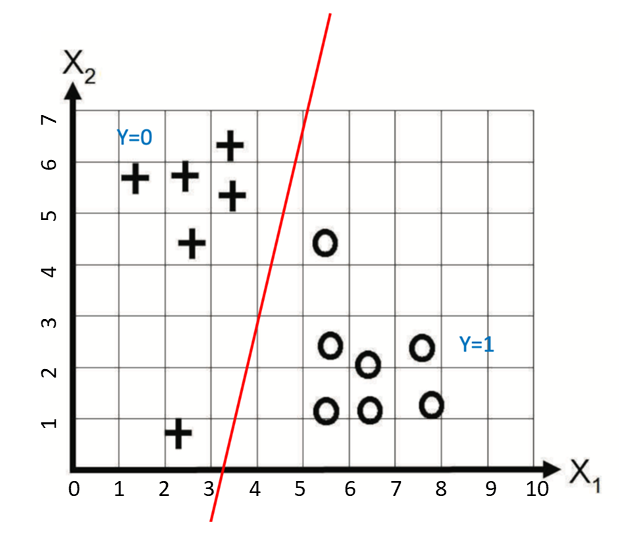
\includegraphics[scale=0.4]{HW2_Q1.png}
\caption{Training data}
\label{fig:db}
\end{figure}

\begin{enumerate}
\item {[2 pts]} Find the training sample with the highest probability of class $1$. Find the training sample
with the highest probability of class $0$. You may specify the sample using co-ordinates or the value range of $X_1$ and $X_2$. Provide brief justification of your answer.

\begin{tcolorbox}[fit,height=3cm, width=15cm, blank, borderline={1pt}{-2pt},nobeforeafter]
%solution

\end{tcolorbox}
\item {[5 pts]}
Use a linear equation to describe the decision boundary (red line) in Figure 1.

\begin{tcolorbox}[fit,height=1cm, width=15cm, blank, borderline={1pt}{-2pt},nobeforeafter]
%solution

\end{tcolorbox}
\item {[3 pts]}
Consider modifying this classifier so that it uses only feature $X_1$. 
Provide the equation for this decision boundary.
Consider modifying this classifier so that it uses only feature $X_2$. 
Provide the equation for this decision boundary.
Which of the two classifiers will perform better on the training data? Provide justification.

\begin{tcolorbox}[fit,height=3cm, width=15cm, blank, borderline={1pt}{-2pt},nobeforeafter]
%solution

\end{tcolorbox}

\item {[5 pts]}
Consider using decision tree on the data in Figure \ref{fig:db}, instead of logistic regression. 
What is the advantage and disadvantage of decision tree over logistic regression?

\begin{tcolorbox}[fit,height=3cm, width=15cm, blank, borderline={1pt}{-2pt},nobeforeafter]
%solution

\end{tcolorbox}

\item {[5 pts]}
Consider using Naive Bayes classifier and decision tree on the data in Figure \ref{fig:db}.
What is the advantage and disadvantage of Naive Bayes over logistic regression?

\begin{tcolorbox}[fit,height=3cm, width=15cm, blank, borderline={1pt}{-2pt},nobeforeafter]
%solution

\end{tcolorbox}

\end{enumerate}

\item {[Logistic Regression, Implementation 10 pts]}
This problem is graded with Autograder.
Follow the below instruction, and implement in \textbf{reg.py}.\\
Do not rename this files, and do not change anything other than the functions you are asked to implement. Otherwise, Autograder might unable to grade your work properly. You are only allowed to use Numpy in this problem.


In this part, you need to train a linear binary classification model $F(x) = \langle w, x \rangle$ with logistic regression (for simplicity, the bias term $b$ is omitted here). For training samples $\{ (x_i, y_i) \}_{i=1}^n$ where $x_i \in \R^d$ and $y_i \in \{ 0,1 \}$, you need to find a vector $w \in \R^d$ that minimizes the following loss function:
\[
    \ell(w) = \frac{1}{n} \sum_{i=1}^n  \left [  \log (1 + e^{\langle w, x_i \rangle}) - y_i \cdot \langle w, x_i \rangle \right ]
\]

which is the negative log likelihood. Minimizing this loss function is a convex optimization problem, which means that in most cases, there exists a unique minimizer. Here, you need to find this minimizer with gradient descent, which runs as follows:
\begin{algorithm}[!htb]
\caption{Gradient Descent}
\begin{algorithmic}
\Require Learning rate $\eta > 0$, stopping criterion $\rho > 0$
\State Initialize $w$
\While{True}
    \State Compute gradient $\nabla_w \ell(w)$
    \State If $\| \nabla_w \ell(w) \| < \rho$ then break
    \State $w \gets w - \eta \cdot \nabla_w \ell(w)$
\EndWhile
\end{algorithmic}
\end{algorithm}

\textbf{Task:} In \texttt{reg.py}, implement three functions: \texttt{compute\_loss} for computing $\ell(w)$, \texttt{compute\_grad} for computing $\nabla_w \ell(w)$, and \texttt{train} for training the model with gradient descent. 



\item {[Decision Tree, 20 pts]} A group of students ran several experiments to design a system to determine the effectiveness of initial drug screening campaign. Your friend took notes on the 8 experiments he has ran, and he wants to construct a decision tree that would predict whether or not drug has effect based on 3 binary features:
\begin{itemize}
    \item $x_1=$ The drug molecule has benzene ring
    \item $x_2=$ The drug molecule has more than 2 negative ions
    \item $x_3=$ The drug molecule showed less than 2 angstrom distance from pocket
\end{itemize}

\begin{center}
\begin{tabular}{c|c c c |c}
\hline
    Movie &$x_1$&$x_2$ & $x_3$ & Like\\ \hline
    $\bar{x}^{(1)}$ & False & False & True & No\\
    $\bar{x}^{(2)}$ & True & False & True & Yes\\
    $\bar{x}^{(3)}$ & False & False & False & Yes\\
    $\bar{x}^{(4)}$ & False & True & True & Yes\\
    $\bar{x}^{(5)}$ & True & True & True & No\\
    $\bar{x}^{(6)}$ & True & False & False & Yes\\
    $\bar{x}^{(7)}$ & True & True & False & Yes\\
    $\bar{x}^{(8)}$ & False & True & False & Yes\\ \hline
\end{tabular}
\end{center}

\begin{enumerate}[(a)]
    \item {[5 pts]} Use the above dataset to construct a decision tree, where each split is performed on the feature with the highest information gain. Use the following stopping conditions in the decision tree algorithm:
\begin{itemize}
    \item Tree depth is 3
    \item Information gain is 0
\end{itemize}
Output majority label if any of the stopping criteria are met, or a positive label if both classes are equally represented. \textbf{NOTE}: To help you out, the TAs have decided to tell you that the split at the root made by this algorithm will be on the feature $x_3$.

\begin{tcolorbox}[fit,height=7cm, width=15cm, blank, borderline={1pt}{-2pt},nobeforeafter]
%solution

\end{tcolorbox}

\item {[5 pts]} Does your decision tree from previous part minimize the training error? If not, report the smallest training error that a decision tree can achieve on this dataset and draw the decision tree. \\


\begin{tcolorbox}[fit,height=8cm, width=15cm, blank, borderline={1pt}{-2pt},nobeforeafter]
%solution

\end{tcolorbox}


\item {[10 pts]} During recitation, we introduced KL-Divergence to provide another view of information gain. Here we have formal definition of KL-Divergence:\\

Let $p$ and $q$ be two discrete probability distributions defined over the same event space. Formally, for $i$ $\in$ $\{1,...,n\}$, let $p(i)$ be the probability of event $i$ occurring under distribution $p$ and $q(i)$ be the corresponding probability under distribution $q$. The \textbf{Kullback-Leibler (KL) divergence} between $p$ and $q$ is defined as
$$
    D(p\|q) = \sum_{i=1}^n p(i)\log\frac{p(i)}{q(i)}
$$


\textbf{KL-Divergence is proven to have non-negative: $ D(p\|q) \geq 0$ }. Using this, we want to show that information gain is always non-negative. In detail, \\

In a sample $S$, the information gain of a variable $Y$ with respect to a target variable $X$ is the expected reduction in entropy of a target variable $X$ after gaining insight into $Y$:
$$
Gain(S, Y) =H_S(X)-H_S(X \mid Y) 
$$
Show that information gain is always non-negative. Show all steps of your work.

\begin{tcolorbox}[fit,height=8cm, width=15cm, blank, borderline={1pt}{-2pt},nobeforeafter]
%solution

\end{tcolorbox}

\end{enumerate}

\item {[K-Means Clustering, 50 pts]} In this homework problem, you will implement $K$-means algorithm and apply it to cluster genes using the
mouse gene expression data from three brain tissue types, HIP, PFC, and STR. For each tissue type, data are provided in two files,
one for expression data, where the rows are for mice/samples and the columns are for genes, and the other file for gene names.
Answer the following questions on the tissue type HIP.
Exlore PFC and STR in the bonus problem.

\textbf{Note:} For ploting the correlation coefficient matrix you can use the pyplot function imshow(). For parts (c) and (d) you should show all the correlation coefficient matrices in one plot. You can achieve this with the pyplot.subplots() function. Each subplot should be titled with the objective function value (parts (c) and d) and the K value (part (d) only).

\begin{enumerate}
\item{[15 pts]} Run $K$-means algorithm with $K=3$ with the initialization of $K$ means given in `test\_mean.txt'. Plot the objective ($y$-axis)
over iterations ($x$-axis). What is the objective value at convergence? (Make sure you use the given initialization. The initialization is given
for the grading purpose.)

\begin{tcolorbox}[fit,height=6cm, width=15cm, blank, borderline={1pt}{-2pt},nobeforeafter]
%solution

\end{tcolorbox}

\item {[10 pts]} Run $K$-means algorithm with $K=3$ with your own random initialization. 
Plot the correlation coefficient matrix of a) the raw data
and b) the data after you group the columns of the expression matrix according to the clusters found by K-means.
Plot these as an image of $N\times N$ correlation matrix for $N$ genes.

\begin{tcolorbox}[fit,height=6cm, width=15cm, blank, borderline={1pt}{-2pt},nobeforeafter]
%solution

\end{tcolorbox}

\item {[10 pts]} With $K=3$, try 10 random initializations. Show the correlation coefficient matrix as above
and the corresponding objective at convergence for each initialization. Which of the 10 results would you choose for follow-up analysis?

\begin{tcolorbox}[fit,height=6cm, width=15cm, blank, borderline={1pt}{-2pt},nobeforeafter]
%solution

\end{tcolorbox}

\item {[15 pts]} Run K-means algorithm for $K=3,\ldots, 12$, with 10 random initializations for each $K$.
Show the correlation coefficient matrix and objectives at convergence for different $K$, with your best choice of
the 10 runs for each $K$. What do you think is the best $K$? Why?

\begin{tcolorbox}[fit,height=6cm, width=15cm, blank, borderline={1pt}{-2pt},nobeforeafter]
%solution

\end{tcolorbox}
\end{enumerate}


\end{enumerate}



\end{document}
